\documentclass[aspectratio=169]{beamer}
\usetheme{metropolis}
\usepackage{graphicx}
\usepackage{amsmath}
\usepackage{amssymb}
\usepackage{booktabs}

\title{Representation Learning with Autoencoders}
\subtitle{AE \& $\beta$-VAE on Medical MNIST \\ DSAI 490 -- Assignment 1}
\author{Amr Yasser}
\date{\today}

\begin{document}

\maketitle

% ---------------------------------------------------------------
\begin{frame}{Problem and dataset}
  \textbf{Goal.} Compare a convolutional Autoencoder and a convolutional $\beta$-Variational Autoencoder on real medical images, measuring reconstruction, latent structure, generation, and denoising.

  \vspace{0.6em}
  \textbf{Dataset.} Medical MNIST -- 6 classes of $64{\times}64$ grayscale scans: AbdomenCT, BreastMRI, CXR, ChestCT, Hand, HeadCT.

  \vspace{0.6em}
  \textbf{Pipeline.} \texttt{tf.data} -- JPEG decode $\to$ resize $\to$ $[0,1]$ scale $\to$ shuffle $\to$ batch 128 $\to$ prefetch. Split $80/10/10$ train/val/test.

  \vspace{0.6em}
  \textbf{Training.} Keras functional API, Adam ($10^{-3}$), \textbf{30 epochs}, single Kaggle GPU.
\end{frame}

% ---------------------------------------------------------------
\begin{frame}{Sample images and classes}
  \centering
  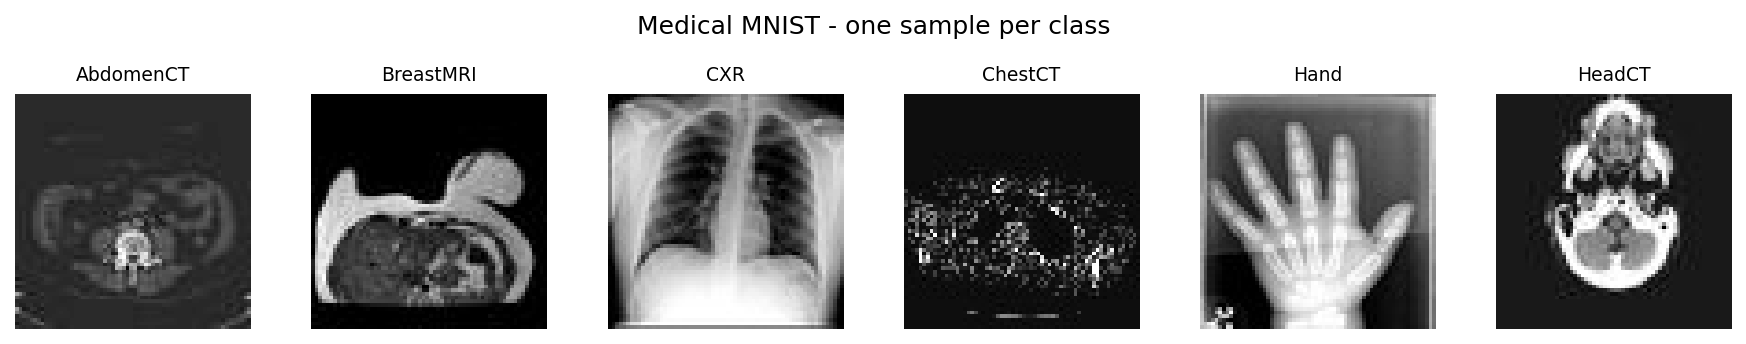
\includegraphics[width=\linewidth]{../figures/01_dataset_samples.png}

  \vspace{0.4em}
  \small Six visually distinct modalities and anatomies. CXR and ChestCT are most similar to each other; the others are well-separated.
\end{frame}

% ---------------------------------------------------------------
\begin{frame}{Architectures -- AE vs $\beta$-VAE}
  \begin{columns}[T]
    \column{0.5\textwidth}
    \textbf{Autoencoder}
    \begin{itemize}
      \item \texttt{Conv2D} + \texttt{MaxPool} $\times 3$ ($32{\to}16{\to}16$)
      \item Bottleneck: $8{\times}8{\times}16 = 1024$ dims
      \item \texttt{Conv2DTranspose} $\times 3$, stride 2
      \item Sigmoid output head
      \item Loss: pixelwise BCE
      \item Deterministic, unregularised
    \end{itemize}

    \column{0.5\textwidth}
    \textbf{$\beta$-VAE}
    \begin{itemize}
      \item Strided \texttt{Conv2D} ($32{\to}64{\to}64$) + dense 128
      \item Two heads $\to (\boldsymbol{\mu}, \log \boldsymbol{\sigma}^2) \in \mathbb{R}^{16}$
      \item Reparameterise $\mathbf{z}=\boldsymbol{\mu}+\boldsymbol{\sigma}\odot\boldsymbol{\epsilon}$
      \item Symmetric \texttt{Conv2DTranspose} decoder
      \item Loss: BCE $+\;\beta \cdot \mathrm{KL}(q\,\|\,\mathcal{N}(0,I))$
      \item Probabilistic, prior-regularised
    \end{itemize}
  \end{columns}
\end{frame}

% ---------------------------------------------------------------
\begin{frame}{Why $\beta = 0.25$ and not $\beta = 1$?}
  The standard ELBO uses $\beta = 1$. On this dataset, that caused \emph{partial posterior collapse}:
  \begin{itemize}
    \item KL dropped to $\approx 27$ nats (encoder hugging the prior)
    \item Reconstructions were severely blurred
    \item The encoder gave up information to minimise KL
  \end{itemize}

  \vspace{0.6em}
  Lowering $\beta$ to $0.25$ lets the encoder carry more information:
  \begin{itemize}
    \item KL rose to $\approx 43$ nats (counter-intuitive but correct: lower $\beta$ $\Rightarrow$ \emph{higher} KL at equilibrium)
    \item Reconstruction BCE dropped from $\sim 1970$ to $\sim 1900$
    \item Generation and denoising both improved
  \end{itemize}

  \vspace{0.5em}
  This is $\beta$-VAE (Higgins et al., 2017), with $\beta<1$ favouring reconstruction.
\end{frame}

% ---------------------------------------------------------------
\begin{frame}{Training dynamics}
  \begin{columns}[T]
    \column{0.32\textwidth}
    \centering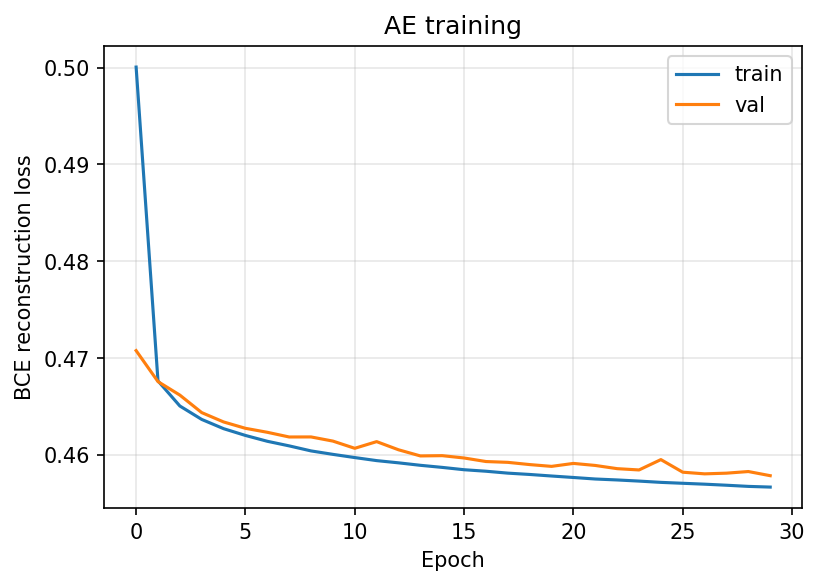
\includegraphics[width=\linewidth]{../figures/02_ae_loss.png}\\
    \scriptsize \textbf{AE.} BCE $0.50\!\to\!0.46$, plateau after $\sim$20 epochs.
    \column{0.66\textwidth}
    \centering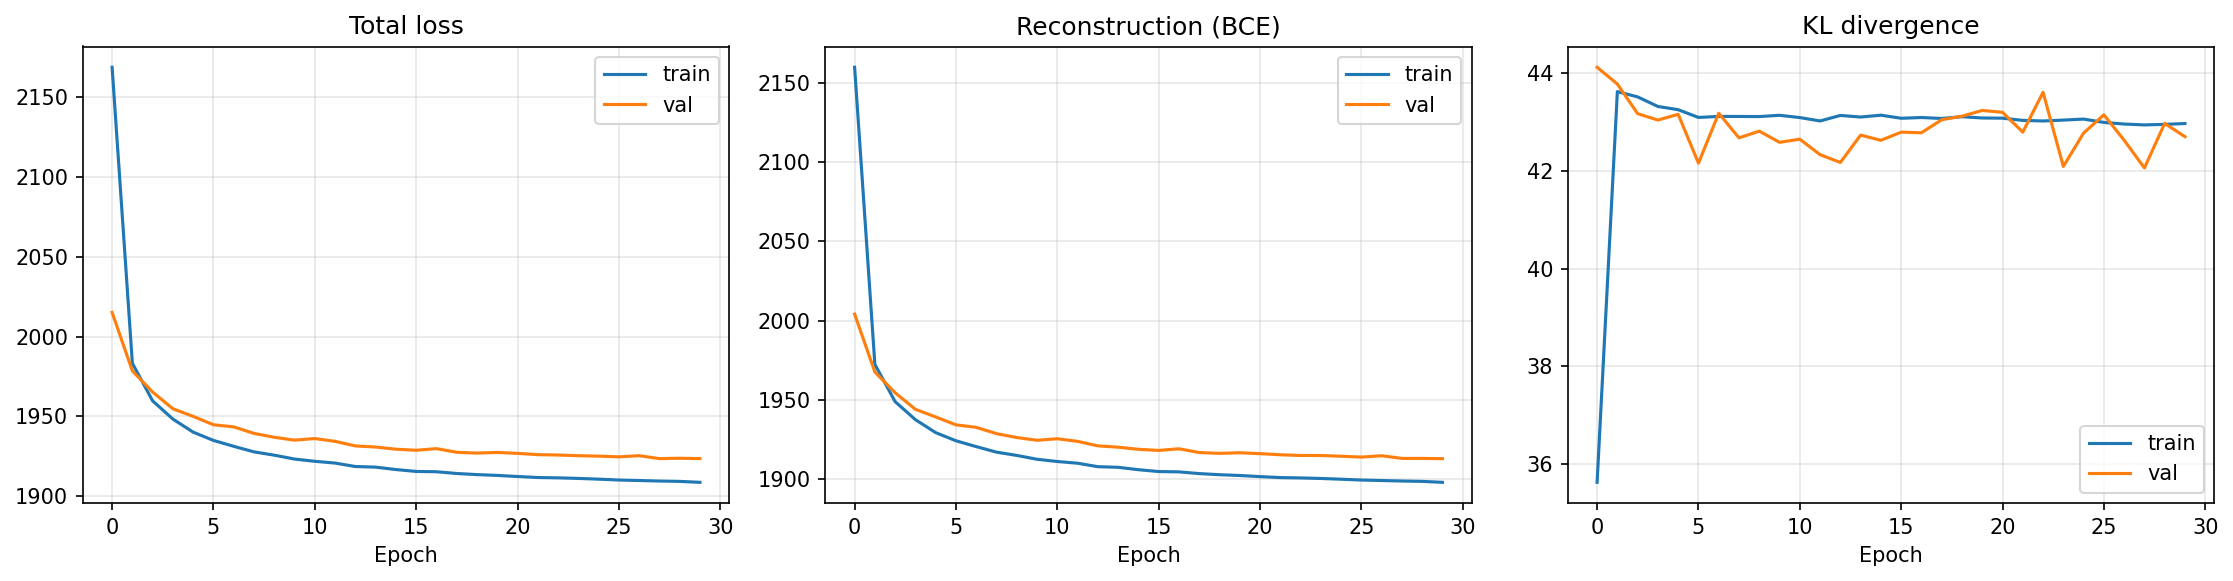
\includegraphics[width=\linewidth]{../figures/03_vae_loss.png}\\
    \scriptsize \textbf{$\beta$-VAE.} Reconstruction drops $2160\!\to\!1900$; KL settles at $\sim$43 nats. Encoder carrying information, not collapsing.
  \end{columns}
\end{frame}

% ---------------------------------------------------------------
\begin{frame}{Reconstruction: AE vs $\beta$-VAE}
  \centering
  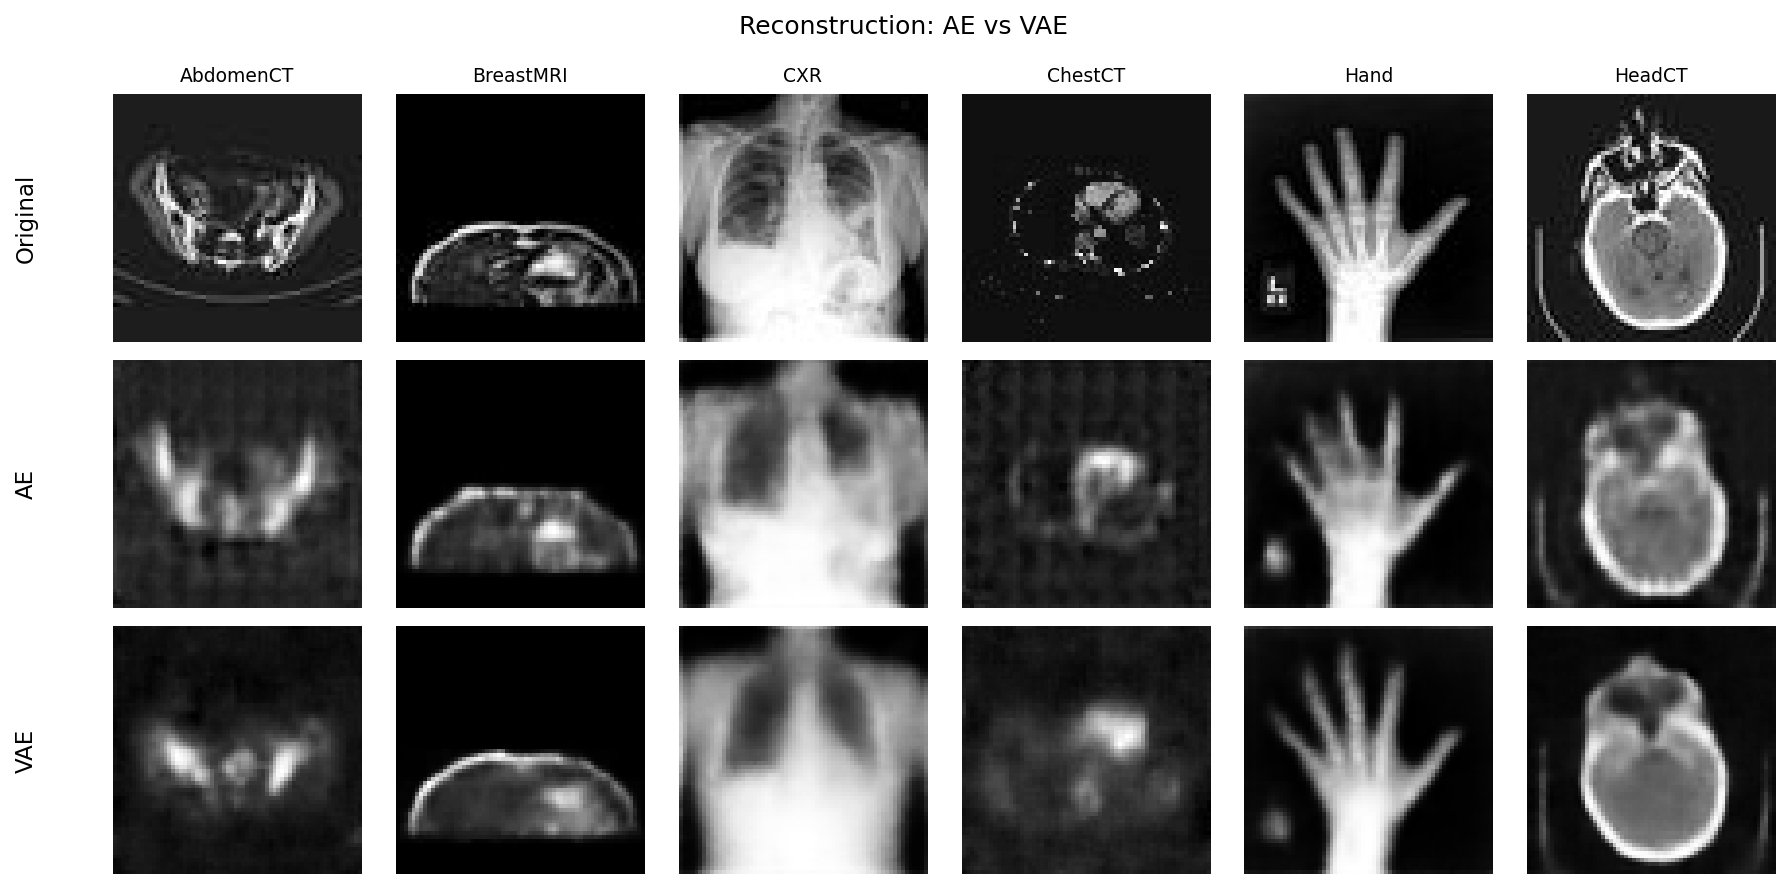
\includegraphics[width=0.88\linewidth]{../figures/04_reconstruction_comparison.png}

  \vspace{0.3em}
  \scriptsize Both preserve global anatomy. AE preserves slightly more texture (1024-dim code). $\beta$-VAE output is smoother -- the ``VAE blur,'' driven by the 16-dim KL-regularised code.
\end{frame}

% ---------------------------------------------------------------
\begin{frame}{Reconstruction metrics}
  \centering
  \begin{tabular}{lcc}
    \toprule
                  & \textbf{Test MSE} & \textbf{Test MAE} \\
    \midrule
    AE            & $0.00429$ & $0.0355$ \\
    $\beta$-VAE   & $0.00699$ & $0.0449$ \\
    \bottomrule
  \end{tabular}

  \vspace{1em}
  \begin{itemize}
    \item AE wins on pixel error by $\approx 39\%$ -- expected: 1024 free dimensions, no KL regulariser.
    \item VAE ``loses'' by design: 16 regularised dimensions + explicit pull toward the prior.
    \item Low numbers are misleading on their own -- MSE is dominated by the large black backgrounds.
  \end{itemize}
\end{frame}

% ---------------------------------------------------------------
\begin{frame}{Latent-space structure}
  \centering
  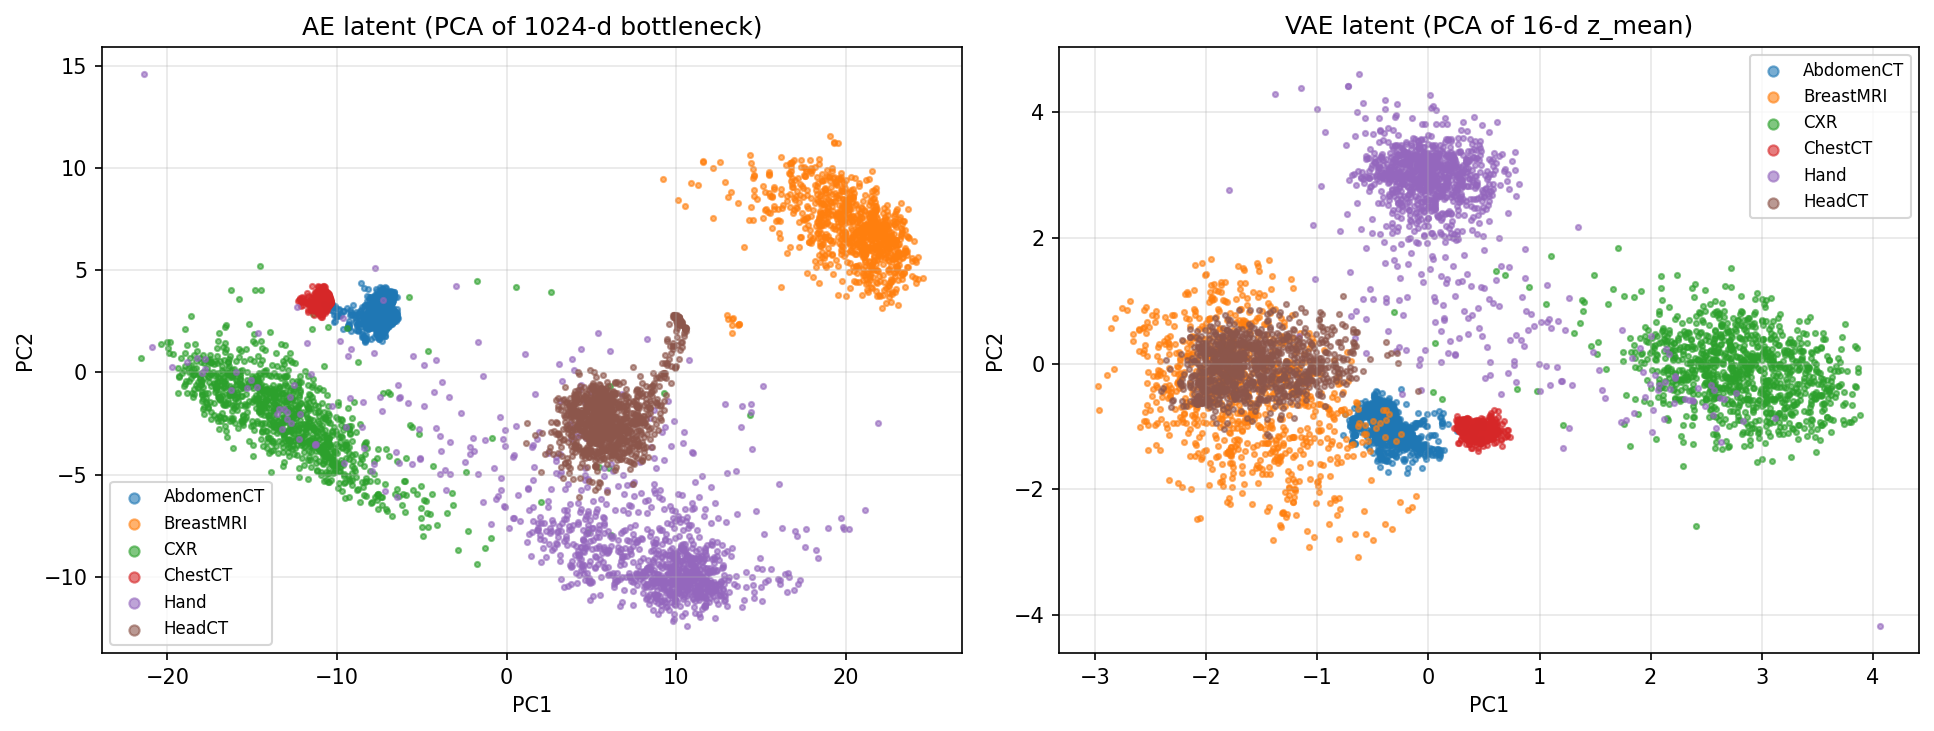
\includegraphics[width=0.88\linewidth]{../figures/05_latent_space_pca.png}

  \vspace{0.3em}
  \scriptsize \textbf{AE (left).} Tight, well-separated class clusters -- good for a downstream classifier.\quad
  \textbf{$\beta$-VAE (right).} Compact, origin-centered, more overlap -- the KL pull, but densely populated where the prior puts mass.
\end{frame}

% ---------------------------------------------------------------
\begin{frame}{Sampling from the VAE prior}
  \begin{columns}[T]
    \column{0.50\textwidth}
    \centering
    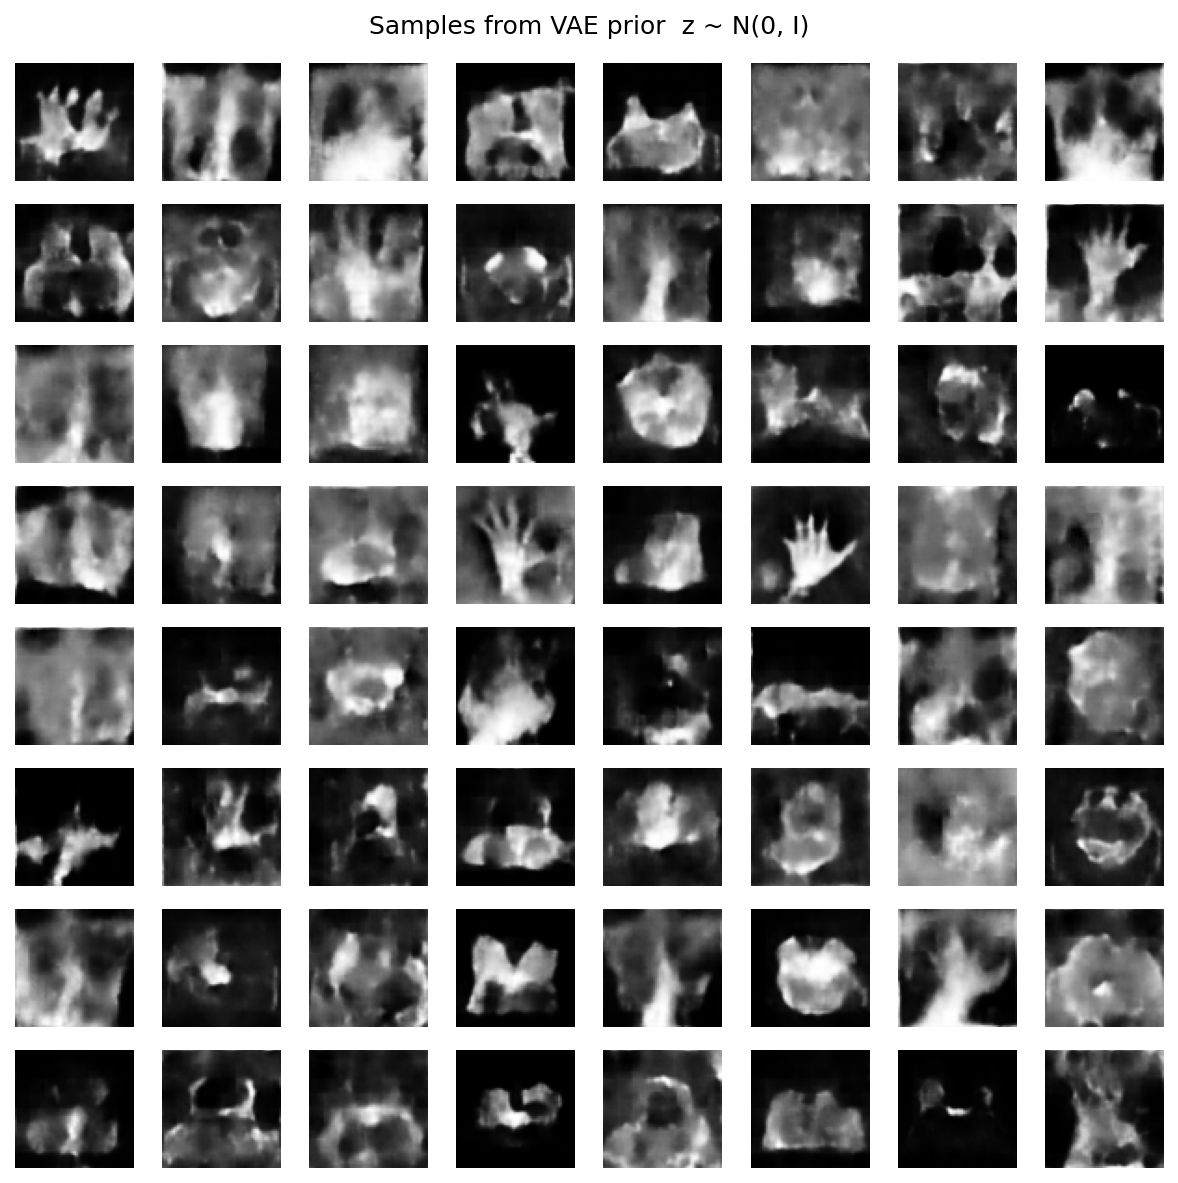
\includegraphics[width=\linewidth]{../figures/06_vae_generated_samples.png}\\
    \scriptsize 64 samples, $z\sim \mathcal{N}(0, I)$
    \column{0.50\textwidth}
    \vspace{0.4em}\small
    \begin{itemize}
      \item Hands and chest silhouettes \emph{recur} across the grid -- real class structure learned in the prior.
      \item Samples are blurry (small latent + Gaussian likelihood, not a training issue).
      \item Sharper synthesis would require VQ-VAE or diffusion at much higher cost.
    \end{itemize}
  \end{columns}
\end{frame}

% ---------------------------------------------------------------
\begin{frame}{Latent interpolation}
  \centering
  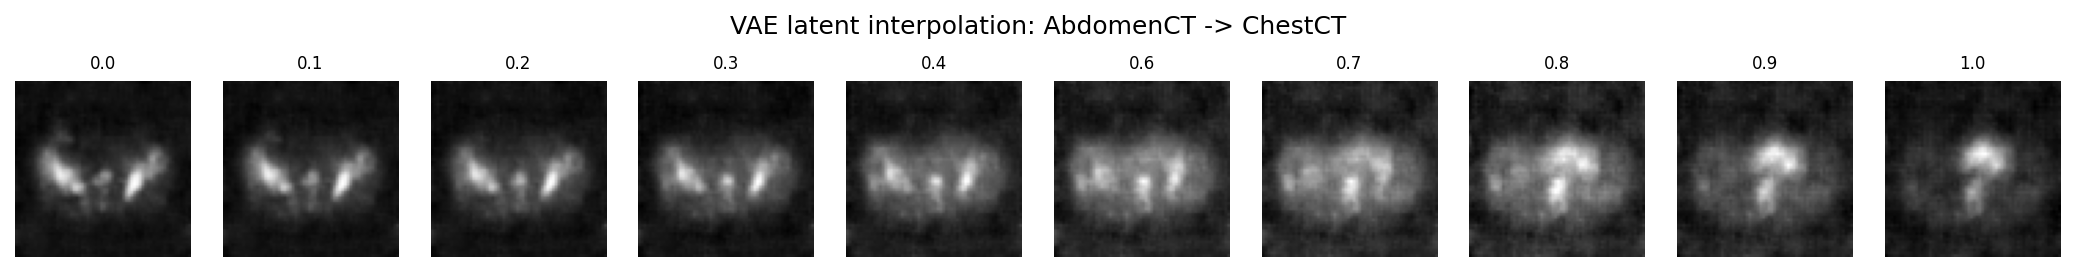
\includegraphics[width=\linewidth]{../figures/07_vae_interpolation.png}

  \vspace{0.4em}
  \small Linear interpolation in $\boldsymbol{\mu}$-space between an AbdomenCT and a ChestCT encoding. Smooth pixel-level transitions (no jumps) confirm the latent manifold is continuous -- a prerequisite for semantic editing. Intermediate frames are visually ambiguous on this dataset.
\end{frame}

% ---------------------------------------------------------------
\begin{frame}{Denoising -- emergent, without retraining}
  \centering
  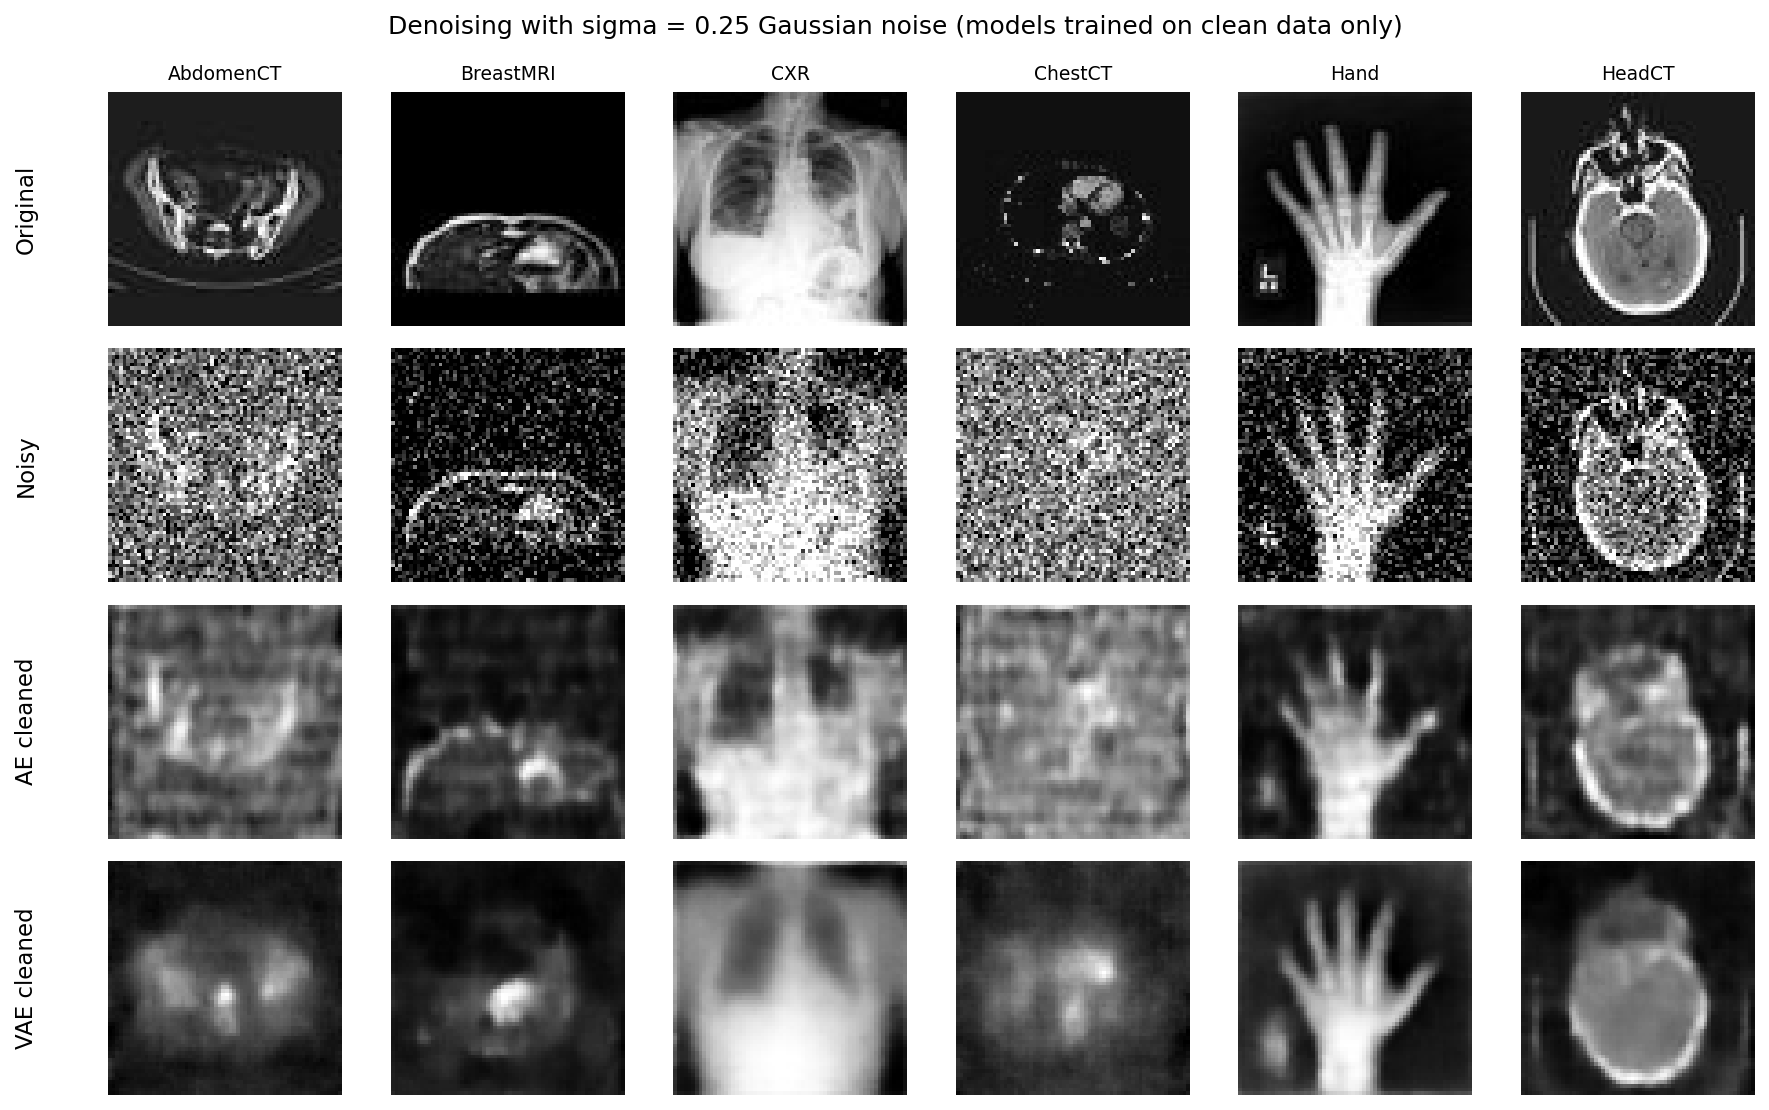
\includegraphics[width=0.82\linewidth]{../figures/08_denoising.png}

  \vspace{0.3em}
  \scriptsize Both models trained on clean data only; fed inputs with $\sigma = 0.25$ Gaussian noise. \\
  \textbf{$\beta$-VAE outperforms the AE} -- the prior-regularised latent is a stronger implicit smoother.
\end{frame}

% ---------------------------------------------------------------
\begin{frame}{Key findings}
  \begin{enumerate}
    \item \textbf{AE and $\beta$-VAE are not interchangeable.} They optimise different objectives.
    \item \textbf{AE wins on reconstruction \& classification.} $39\%$ lower MSE, tighter class clusters in latent space.
    \item \textbf{$\beta$-VAE wins on generation \& denoising.} Only model that can sample; cleaner denoising thanks to the regularised latent.
    \item \textbf{$\beta$-tuning matters.} Standard $\beta{=}1$ caused partial posterior collapse on this dataset; $\beta{=}0.25$ fixed it.
    \item \textbf{Counter-intuitive fact.} Lowering $\beta$ \emph{raises} the equilibrium KL -- the encoder is allowed to carry information.
  \end{enumerate}
\end{frame}

% ---------------------------------------------------------------
\begin{frame}{Limitations and future directions}
  \begin{itemize}
    \item \textbf{Small latent + Gaussian prior is a ceiling for sample sharpness.} VQ-VAE, hierarchical VAEs, or diffusion models would sharpen generation.
    \item \textbf{Denoising was emergent, not trained.} A noise-conditioned denoising AE (noisy input, clean target) would outperform both models for this specific task.
    \item \textbf{Medical MNIST is easy.} Classes are visually distinct, sizes are small. Conclusions do not directly transfer to full-resolution clinical imaging.
    \item \textbf{No perceptual loss.} Pixel BCE underweights structural detail. Using a perceptual loss (e.g.\ from a pretrained classifier) would likely improve both AE and VAE reconstructions.
  \end{itemize}
\end{frame}

\end{document}
